\documentclass[UTF8,a4paper,11pt]{ctexart}
\usepackage[margin=2.0cm]{geometry}
\usepackage{amsmath,amssymb,bm}
\usepackage{booktabs}
\usepackage{graphicx}
\usepackage{caption}
\usepackage{placeins}
\usepackage{hyperref}
\hypersetup{colorlinks=true,linkcolor=blue,urlcolor=blue}
\setlength{\parindent}{2em}
\setlength{\parskip}{0.25em}
\newcommand{\NL}{N_{\mathrm L}}
\newcommand{\NF}{N_{\mathrm F}}
\newcommand{\Pe}{P_{\mathrm{e2e}}}
\newcommand{\Rbar}{\overline R_{\mathrm{cl}}}

\title{密集跟随式 LEO 网络部署优化与资源一致性结果分析}
\author{基于固定总带宽、功率公平性与相关干扰的数值研究}
\date{\today}

\begin{document}
\maketitle

\begin{abstract}
本报告在原 follower-based LEO 随机几何复现和资源一致 SINR 模型基础上，进一步回答
``在网络密集、存在集群间干扰且资源有限时，每个 leader 应部署多少 followers''。
与只增加卫星数量并累加链路速率的比较不同，本文显式区分固定单星功率与固定集群总功率，
令地面总带宽在 cluster 内正交划分，并在固定链路总发射功率口径下令热噪声随分支带宽
缩放。部署优化使用 Wilson 95\% 端到端覆盖下界、独立随机种子复验、独立样本上的
3\% 近最优速率重选，以及完整几何共享复用颜色审计，报告统计稳健的简约 follower 数量
$N_{\rm F}^{\dagger}$。结果表明，followers 的结论
高度依赖功率口径：固定单星功率下，followers 同时增加总功率，平均速率和高门限覆盖
均可显著提高；固定集群总功率下，followers 仍可提高可靠性，但平均速率随数量增加而
下降。共享复用颜色显著提高跨 RB 干扰相关性，follower 可用率同时改善服务分集并增加
外部 follower 干扰，因此可靠性不保证单调增长。
\end{abstract}

\section{分析口径与可复现判据}

部署研究使用详细理论报告
\texttt{resource\_consistent\_sinr\_full\_derivation\_v1.tex} 中的模型。系统总地面带宽为
$B_{\rm tot}$，复用因子为 $K$，因此单 cluster 可用带宽为
\begin{equation}
 B_{\rm cl}=\frac{B_{\rm tot}}{K}.
\end{equation}
若 leader 获得比例 $\alpha$，对称 followers 平分其余带宽，则
\begin{equation}
 B_{\rm LU}=\alpha B_{\rm cl},\qquad
 B_{{\rm FU},i}=\frac{1-\alpha}{\NF}B_{\rm cl}.
\end{equation}
部署图采用固定链路总发射功率和带宽缩放热噪声。以 $B_{\rm tot}$ 为参考带宽，分支噪声
归一化因子为
\begin{equation}
 \nu_{\rm L}=\frac{\alpha}{K},\qquad
 \nu_{{\rm F},i}=\frac{1-\alpha}{K\NF},
\end{equation}
从而 $\alpha$ 不仅改变 Shannon 速率前的带宽因子，也改变 SINR 分母中的热噪声。
这一口径适用于链路总发射功率固定、带宽变窄时功率集中到更窄 RB 的情形。若实际系统
采用固定功率谱密度，则必须重新缩放信号和干扰功率，不能直接套用本文最优分配结论。

部署相图不是直接选择样本均值最大的点。首先要求扫描样本的 Wilson 95\% 覆盖下界满足
\begin{equation}
 P_{\mathrm{e2e}}^{\mathrm{L},95\%}\geq0.99.
\end{equation}
然后在独立随机种子和更大样本下重新计算每个 follower 数量的最佳候选、可行集合与
可行最大平均速率 $R_{\max,\rm val}^{\rm feas}$，并在满足
\begin{equation}
 \overline R_{\rm cl,val}\geq0.97R_{\max,\rm val}^{\rm feas}
\end{equation}
的候选中选择最小 $\NF$，得到简约部署候选。最后使用完整几何 Monte Carlo、共享复用
颜色和新的随机种子审计该候选；若其 Wilson 覆盖下界低于 $0.99$，则顺次审计下一候选。
因此，$N_{\rm F}^{\dagger}$ 的含义是：在 $\gamma=-5$ dB 的高可靠约束下，经过独立
速率重选和相关干扰覆盖审计后，以不超过 3\% 的验证速率代价减少硬件数量。
此外，独立的多随机种子审查报告每个场景的重复选择范围；当该范围包含多个离散值时，
工程结论应写成近最优部署区间，而不是唯一精确整数。
这里的“近最优”严格限定于代码公开记录的有限候选集合：
\[
 \NF\in\{0,2,5,10,15,20,30\},\qquad
 \alpha\in\{0.2,0.35,0.5,0.65,0.8\}
\]
并额外包含均匀分配与 leader 保底候选。D2 对不同 $K$、$G_{\rm I}$ 和
$p_{\rm act}$ 分别生成场景曲线，但不把它们与功率比例同时作为连续变量联合求解；
固定集群总功率场景的 leader 功率比例为 $0.5$。因此本文报告的是有限网格上的统计稳健
简约解，而不是连续设计空间中的无条件全局最优解。

\section{带宽分配策略}

\begin{figure}[htbp]
\centering
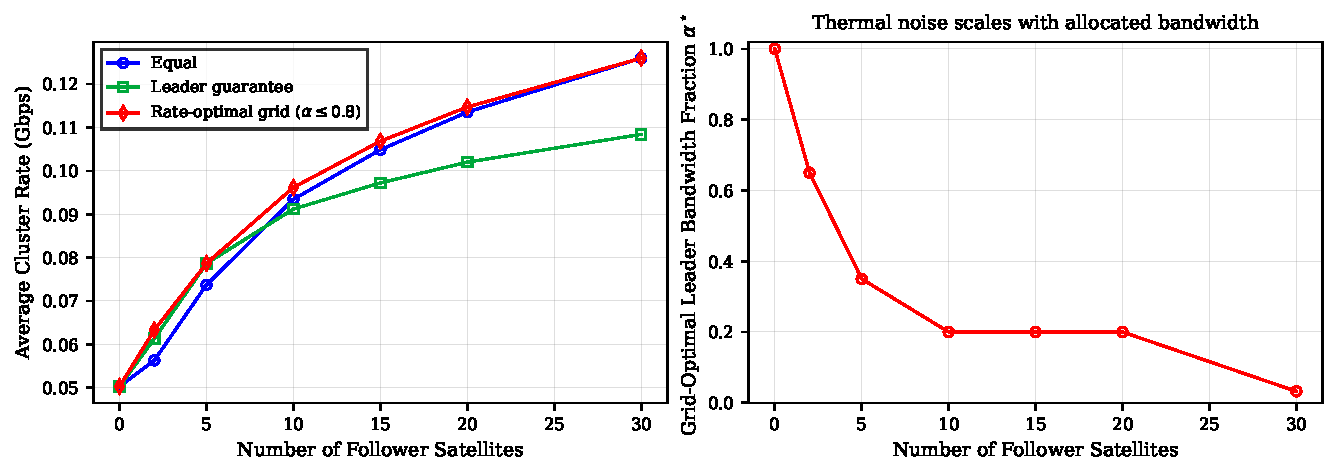
\includegraphics[width=0.98\linewidth]{../figures/deployment/figD1_allocation_strategies.pdf}
\caption{均匀分配、leader 保底分配与网格速率最优分配。部署诊断采用固定单星功率。}
\label{fig:d1}
\end{figure}

图 \ref{fig:d1} 左图比较三种对称带宽分配。$\NF=0$ 时 cluster 仅有 leader，平均速率约为
$0.0503$ Gbps。随着 followers 增加，网格速率最优方案在 $\NF=2,5,10$ 时分别选择
$\alpha^\star=0.65,0.35,0.20$；在 $\NF=10$--$20$ 时最优值保持在扫描下界 $0.20$，
而 $\NF=30$ 时均匀分配比例 $1/31$ 略优，因此被纳入候选集并选中。
相应平均速率在 $\NF=2,10,30$ 时约为 $0.0633$、$0.0962$ 和 $0.1260$ Gbps。

这一结果不能单独解释为``followers 在公平资源下总能增加速率''。D1 使用固定单星功率，
每增加一颗 follower 就增加一套地面功放，集群总发射功率随 $\NF$ 增长。与此同时，
带宽缩放噪声使每个窄 follower RB 的热噪声下降。两者共同使 aggregate follower rate
具有竞争力，因此速率最优分配逐渐把更多带宽留给 followers。D1 的作用是证明一般
$\alpha$ 分配和噪声缩放实现正确；功率公平性必须结合 D3 判断。

右图还表明，固定 $\alpha=0.5$ 的 leader 保底策略不是普遍最优：在 follower 数量较大时，
它给 leader 留出的带宽超过速率目标所需，平均 cluster rate 明显低于网格最优方案。
因此工程系统不应把固定 leader 比例视为与网络状态无关的常数。

\FloatBarrier
\section{高可靠约束下的简约 follower 数量}

\begin{figure}[htbp]
\centering
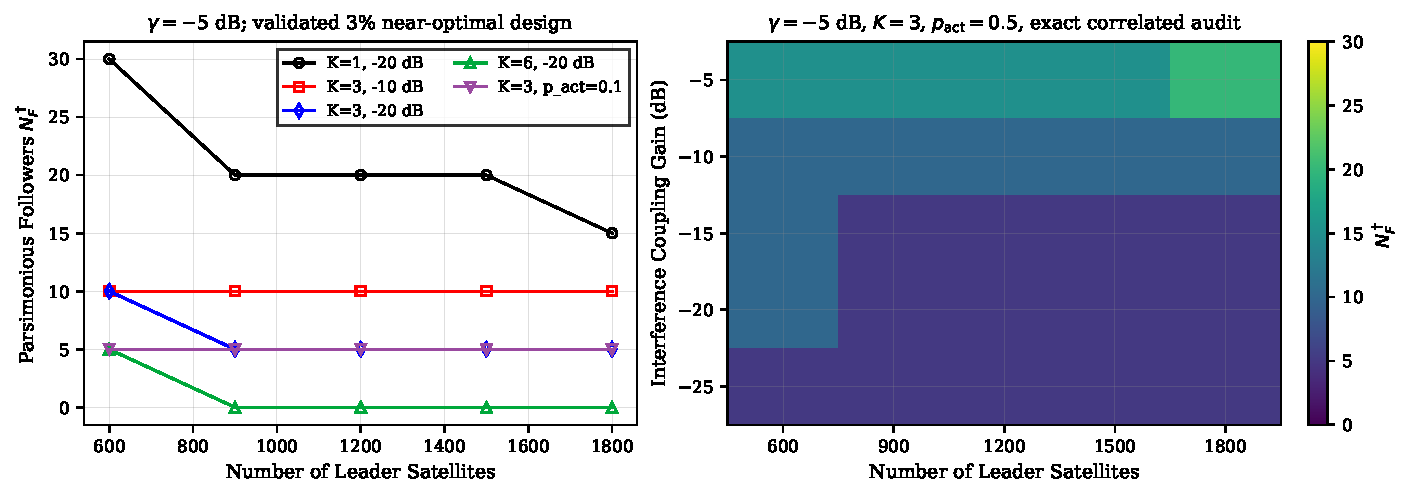
\includegraphics[width=0.99\linewidth]{../figures/deployment/figD2_optimal_follower_phase.pdf}
\caption{固定地面下行集群总功率为 20 dBW 时，高可靠约束下的简约 follower 数量。}
\label{fig:d2}
\end{figure}

图 \ref{fig:d2} 是部署研究的核心结果，覆盖门限为 $\gamma=-5$ dB。所有选中点均在
独立复验样本上重新进入 3\% 近最优速率集合，并通过完整几何、共享复用颜色条件下的
$P_{\mathrm{e2e}}^{\mathrm{L},95\%}\geq0.99$ 门禁；同时使用固定集群总功率，避免把新增
硬件功率误当作架构增益。

在 $K=1,G_{\rm I}=-20$ dB 时，为满足高可靠要求且保持接近最大可行速率，
$N_{\rm F}^{\dagger}$ 在扫描密度内为 $15$--$30$。复用 1 给每个 cluster 完整带宽，
但同频外部 cluster 最多，因此需要较多 followers 提供分集。$K=3,G_{\rm I}=-10$ dB
时，推荐值稳定为 $10$；将耦合进一步降低到 $-20$ dB 后，推荐值从 $\NL=600$ 时的
$10$ 降至密集场景中的 $5$。这说明强隔离减少了为满足同一可靠性目标所需的冗余分支。

当 $K=6,G_{\rm I}=-20$ dB 时，$\NL=600$ 的最终完整相关审计点需要 $5$ 个 followers，
而 $\NL\geq900$ 时 leader-only 已位于 3\% 验证速率容差内并满足覆盖门禁。这里并非宣称
followers 没有可靠性作用，而是高复用和强隔离已经使 leader 分支足够可靠，继续添加
followers 的边际收益不足以抵消功率分割和部署成本。

右侧相图给出更完整的密度--隔离联合影响。弱隔离 $G_{\rm I}=-5$ dB 时通常需要约
$15$--$20$ 个 followers；隔离增强后，大部分区域降至 $5$--$10$。相图并非严格单调，
原因包括最近 leader 距离缩短、外部 cluster 数增加、固定总功率在分支间重分配以及
离散 follower 网格。通过独立速率重选和完整相关覆盖审计后仍保留的跳变应解释为多机制
竞争与离散设计分辨率共同作用，而不是简单线性规律。由于 $N_{\rm F}^{\dagger}$ 仍是
有限候选网格上的统计决策，最终工程部署还应报告重复种子选择频率和邻近候选性能，而不应
把单个格点解释为连续参数空间中的唯一精确最优值。

五次独立重复的稳定性审查进一步量化了这一点：25 个曲线场景中有 14 个每次都选择相同
$\NF$，23 个场景的众数支持率不低于 80\%，最大重复范围宽度为 10 个 followers。
唯一落在边缘矩重复范围之外的最终点是
$K=6,G_{\rm I}=-20$ dB、$\NL=600$：边缘矩重复选择范围为 $0$--$2$，但完整相关审计
连续拒绝两个更小候选，故最终上调到 $5$。这说明相关干扰审计不是装饰性检查，它能够
实质改变高可靠部署的可行集合。

\FloatBarrier
\section{功率一致性改变核心结论}

\begin{figure}[htbp]
\centering
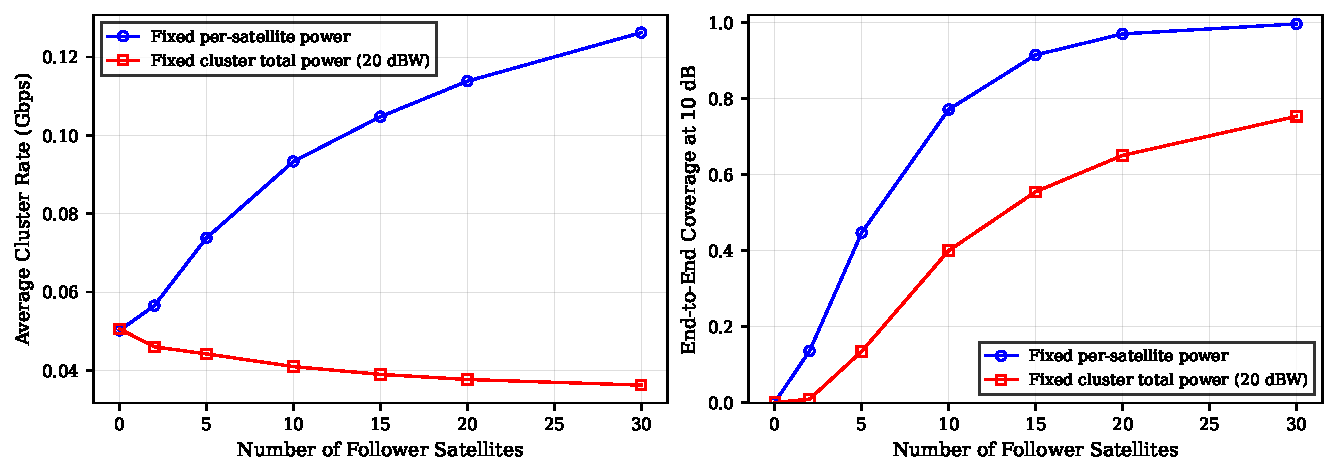
\includegraphics[width=0.98\linewidth]{../figures/deployment/figD3_power_consistency.pdf}
\caption{固定单星功率与固定地面下行集群总功率的速率和 10 dB 端到端覆盖对比。}
\label{fig:d3}
\end{figure}

图 \ref{fig:d3} 证明功率口径不是次要参数，而会改变研究结论的方向。固定单星功率下，
$\NF=0\to30$ 时平均速率由约 $0.0502$ Gbps 增至 $0.1262$ Gbps；10 dB 端到端覆盖
由有限样本中的约 $0.0011$ 增至 $0.9966$。这种增益同时包含空间分集、新增总发射功率
和窄带噪声下降。

固定集群总功率为 20 dBW 时，$\NF=0\to30$ 的平均速率反而由约 $0.0506$ Gbps 降至
$0.0362$ Gbps。原因是 leader 获得一半总功率，另一半再由所有 followers 平分；
followers 数量增加时，单 follower 功率下降，且每条 relay 路径仍受 LF/FU 最小速率
约束。尽管如此，10 dB 端到端覆盖仍由约 $0.0006$ 提升到 $0.7534$，说明 followers
在固定功率下主要提供可靠性，而不是平均速率增益。

因此，任何关于``增加 followers 提升性能''的结论都必须回答：提升的是速率还是可靠性，
并且是否允许集群总功率随卫星数量增加。D2 采用固定集群总功率，正是为了给出更保守、
可比较的部署建议。

\FloatBarrier
\section{高度与 follower 球冠角敏感性}

\begin{figure}[htbp]
\centering
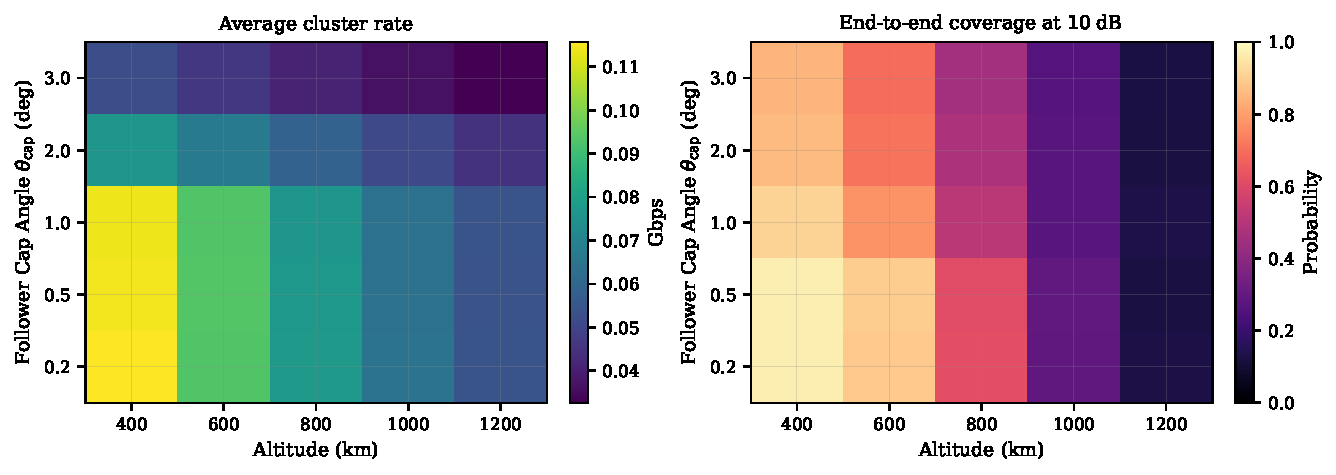
\includegraphics[width=0.98\linewidth]{../figures/deployment/figD4_geometry_sensitivity.pdf}
\caption{轨道高度与 follower 球冠角对平均速率和 10 dB 端到端覆盖的影响。}
\label{fig:d4}
\end{figure}

图 \ref{fig:d4} 表明高度是当前参数域中的主导几何因素。最优扫描点为
$h=400$ km、$\theta_{\rm cap}=0.2^\circ$，平均速率约 $0.1157$ Gbps，10 dB 端到端
覆盖约 $0.9677$。最低平均速率出现在 $h=1200$ km、$\theta_{\rm cap}=3^\circ$，
约为 $0.0326$ Gbps；最低覆盖约为 $0.118$，出现在 1200 km 附近。

高度上升同时增加 leader--user、follower--user 和部分 leader--follower 距离，路径损耗
迅速增加。增大 follower 球冠角可扩大 cluster 的空间分散程度，但也增加 follower 偏离
典型用户和 ISL 距离变大的概率。在当前均匀球冠模型中，较大的球冠角总体降低平均速率；
其影响在高轨道处更加明显。该结论不排除经过用户感知定位或定向调度后的大球冠结构获得
收益，但说明随机均匀扩散本身不是免费的空间分集。

\FloatBarrier
\section{平均值不足以描述边缘性能}

\begin{figure}[htbp]
\centering
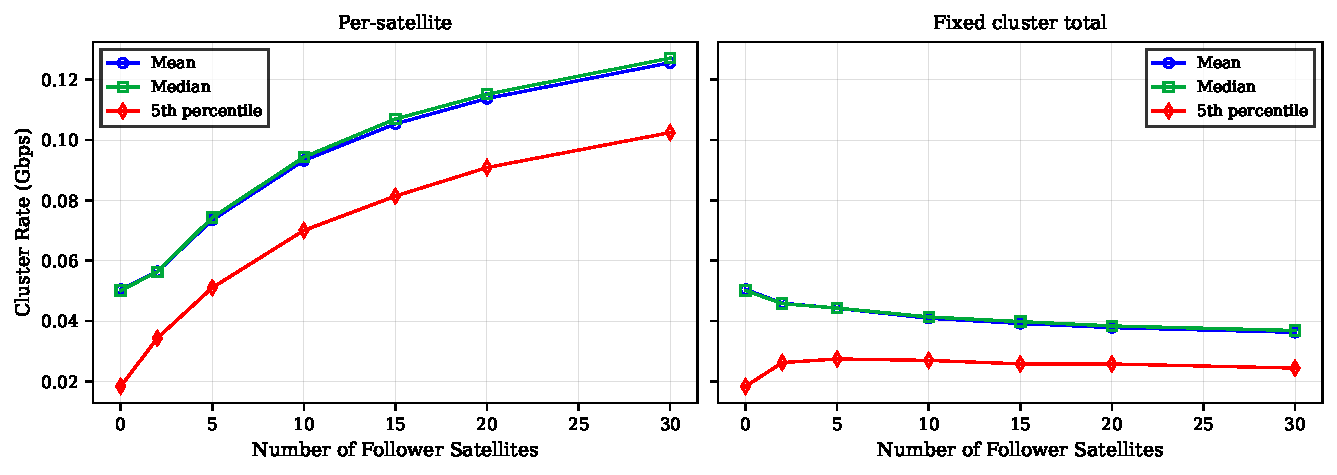
\includegraphics[width=0.98\linewidth]{../figures/deployment/figD5_percentile_rates.pdf}
\caption{两种功率口径下的平均、中位数和 5\% 分位 cluster rate。}
\label{fig:d5}
\end{figure}

图 \ref{fig:d5} 说明平均速率会掩盖低尾用户体验。固定单星功率时，$\NF=30$ 的平均、
中位数和 5\% 分位速率分别约为 $0.1256$、$0.1271$ 和 $0.1025$ Gbps。followers
增加后，低尾速率也显著改善，说明该口径下新增功率和分集同时惠及较差几何样本。

固定集群总功率时，$\NF=30$ 的平均和 5\% 分位速率分别约为 $0.0363$ 和
$0.0244$ Gbps，均低于 leader-only 的平均值。值得注意的是，少量 followers 可使
5\% 分位速率先由约 $0.0184$ 提升到约 $0.027$ Gbps，随后逐渐下降。这说明在固定功率
下，适量 followers 能改善低尾可靠性，但过多 followers 会因功率和带宽分割损害所有
分支。部署设计应同时报告平均值和低分位指标。

\FloatBarrier
\section{共享复用颜色与相关干扰}

\begin{figure}[htbp]
\centering
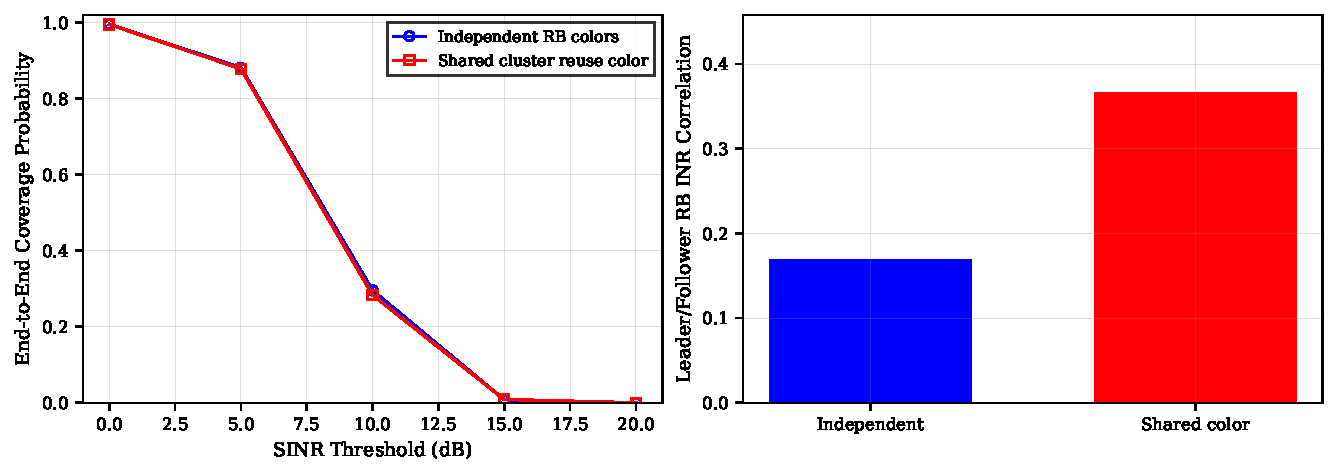
\includegraphics[width=0.98\linewidth]{../figures/deployment/figD6_shared_interference_correlation.pdf}
\caption{独立 RB 颜色与 cluster 级共享复用颜色的覆盖和干扰相关性对比。}
\label{fig:d6}
\end{figure}

图 \ref{fig:d6} 验证了共享外部 cluster 状态不能被简单替换为相互独立的分支干扰。
独立 RB 颜色时，leader RB 与一个 follower RB 的 INR 相关系数约为 $0.1693$；
共享 cluster 复用颜色后升至约 $0.3664$。相关性增加意味着多个服务分支更容易同时经历
较好或较差的外部干扰状态，独立事件乘积会低估联合尾部风险。

在 10 dB 门限处，独立颜色和共享颜色的端到端覆盖分别约为 $0.2955$ 和 $0.2835$。
差异不巨大，但方向稳定：共享干扰状态降低高门限联合覆盖。低门限处两条曲线接近，
说明边缘分布近似仍可用于快速扫描；当研究高可靠尾部或多个分支联合事件时，应使用
共享颜色完整几何模型复验。

\FloatBarrier
\section{Follower 可用率与 ISL 双工代价}

\begin{figure}[htbp]
\centering
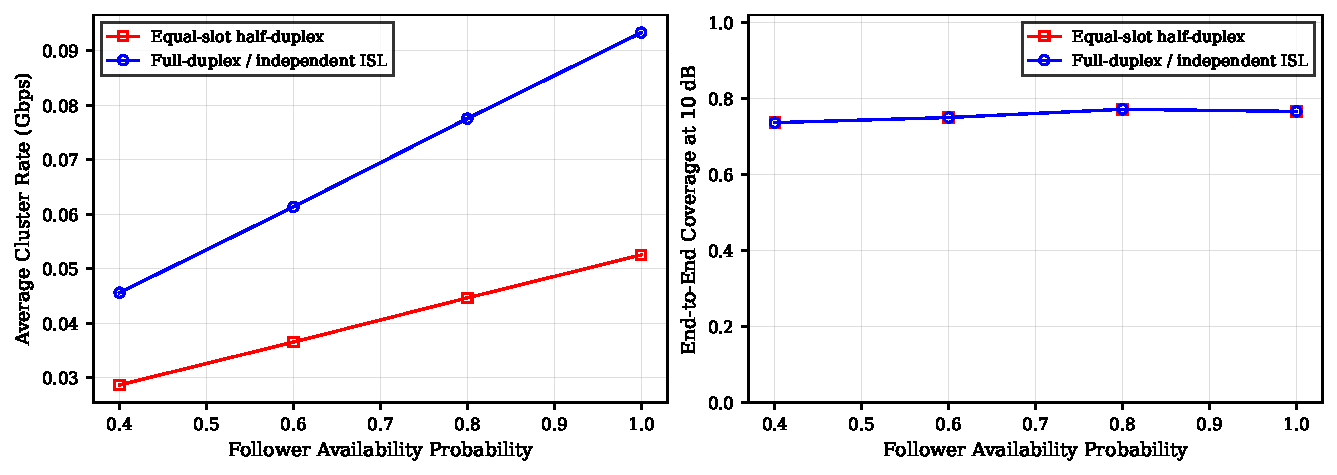
\includegraphics[width=0.98\linewidth]{../figures/deployment/figD7_availability_duplex.pdf}
\caption{Follower 可用概率与 ISL 双工因子对平均速率和 10 dB 端到端覆盖的影响。}
\label{fig:d7}
\end{figure}

图 \ref{fig:d7} 左图显示 follower 可用率从 $0.4$ 增至 $1.0$ 时，全双工/独立 ISL
平均速率由约 $0.0456$ 增至 $0.0933$ Gbps；等时隙半双工由约 $0.0287$ 增至
$0.0525$ Gbps。半双工因子只作用于 relay rate，因此不会改变 SINR 成功事件，右图中
两条覆盖曲线逐点完全重合。

覆盖随可用率并非严格单调：其在 $p_{\rm dep}=0.8$ 时约为 $0.7718$，在
$p_{\rm dep}=1$ 时略降至 $0.7662$。原因是同一个可用概率同时作用于服务 followers
和外部干扰 followers。提高可用率增加可用 relay 分支，但也增加其他 clusters 的
follower 干扰。该结果说明可靠性工程不能只提高卫星在线率，还要配合同频调度和波束
隔离。

\FloatBarrier
\section{最大可见角、集群总功率与 ISL 门限敏感性}

\begin{figure}[htbp]
\centering
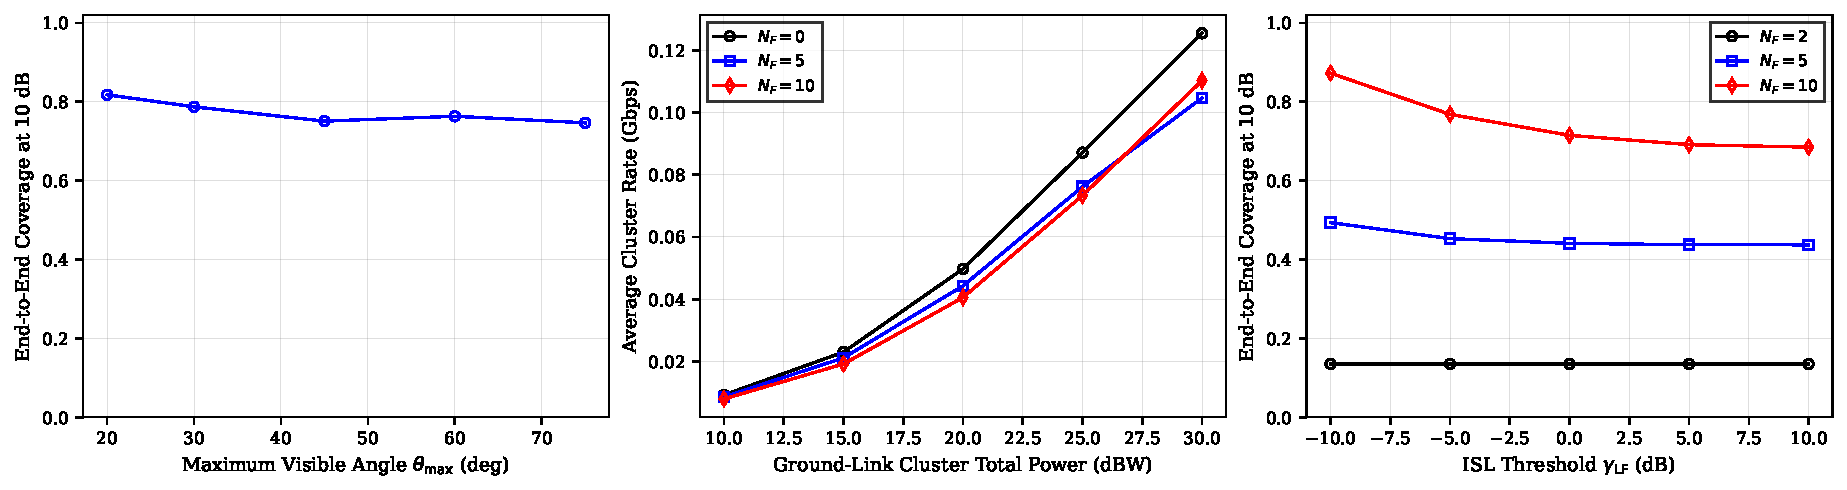
\includegraphics[width=0.99\linewidth]{../figures/deployment/figD8_residual_sensitivity.pdf}
\caption{剩余关键参数敏感性：最大可见角、固定地面下行集群总功率与 ISL 覆盖门限。}
\label{fig:d8}
\end{figure}

图 \ref{fig:d8} 左图考察最大可见接触角 $\theta_{\max}$。在
$\NL=1000,\NF=10$、地面门限为 $10$ dB 的协调场景中，$\theta_{\max}$ 从
$20^\circ$ 增至 $75^\circ$ 时，端到端覆盖由约 $0.8177$ 降至 $0.7466$，平均
cluster rate 由约 $0.0956$ Gbps 降至 $0.0918$ Gbps。扩大可见区域虽然允许更远
服务或干扰卫星进入几何视野，但在最近 leader 服务规则下，主要新增作用是累积更多远端
同频干扰；因此“可见卫星越多越好”并不成立。$60^\circ$ 附近的有限样本轻微起伏不改变
总体下降趋势。

中图采用固定地面下行集群总功率，并比较 $\NF=0,5,10$。总功率由 $10$ dBW 增至
$30$ dBW 时，三种配置的平均速率均显著提高；例如 leader-only 由约 $0.0092$ Gbps
升至 $0.1255$ Gbps，$\NF=10$ 由约 $0.0080$ Gbps 升至 $0.1103$ Gbps。但在相同
总功率和固定总带宽下，高功率区域 leader-only 仍可能获得更高平均速率，因为 followers
需要分割功率与带宽。该结果再次说明 followers 的主要价值应与可靠性目标联合评价，
不能只用平均速率排序。

右图改变 ISL 成功门限 $\gamma_{\rm LF}$。当门限从 $-10$ dB 提高到 $10$ dB 时，
$\NF=2,5,10$ 的端到端覆盖均不增加，其中 $\NF=10$ 从约 $0.8726$ 降至
$0.6849$，下降最明显。原因是 follower 数越多，接入分集越强，但更多候选 relay 路径
同时依赖 LF 解码事件；若忽略 ISL 门限，只报告 FU 接入覆盖，就会系统性高估多 follower
架构的端到端可靠性。

\section{综合设计规则}

由 D1--D8 可得到以下部署规则：
\begin{enumerate}
  \item \textbf{先固定资源口径，再谈 follower 增益。}固定单星功率与固定集群总功率
  会给出相反的平均速率趋势；论文和工程报告必须同时给出两者。
  \item \textbf{高可靠部署应使用置信下界。}D2 使用 Wilson 95\% 下界和独立复验，
  避免把有限样本的偶然高覆盖误判为可行。
  \item \textbf{报告简约解而非脆弱的样本最大值。}若多个 follower 数量的速率差不足
  3\%，优先选择硬件更少的 $N_{\rm F}^{\dagger}$。
  \item \textbf{隔离与复用可以替代部分 follower 冗余。}强隔离和较高复用因子使
  leader-only 或少量 followers 即可满足高可靠目标；弱隔离则需要更多分支。
  \item \textbf{轨道高度通常比随机球冠扩张更重要。}降低高度显著提高速率和高门限
  覆盖；无用户感知的球冠扩张可能增加距离和 ISL 代价。
  \item \textbf{联合可靠性必须保留相关干扰。}公共复用颜色显著增加跨 RB INR
  相关性，高门限联合覆盖应由完整相关模型复验。
  \item \textbf{可用率提升必须与干扰协调同步。}更多在线 followers 同时增加服务
  分集和外部干扰，覆盖不保证单调增加。
  \item \textbf{可见范围和 ISL 门限不能被当作次要参数。}扩大可见区域会引入更多
  远端同频干扰；更严格的 ISL 门限会显著削弱多 follower 端到端可靠性。
\end{enumerate}

\section{结论边界与后续研究}

本研究已经完成资源、功率、统计置信度和最终候选相关干扰审计层面的内部闭环，但结论仍受以下边界
限制。第一，卫星位置采用球面 BPP 快照，不包含真实轨道传播、切换和时间相关性。
第二，干扰隔离使用标量 $G_{\rm I}$，尚未由真实波束图、指向误差、极化和调度联合生成。
第三，固定集群总功率仅指地面下行 LU/FU 功率，独立频段 ISL 功耗未纳入同一能源预算。
第四，网络吞吐仍是典型已调度用户代理，未引入用户点过程、业务到达、排队和时延约束。
第五，带宽缩放噪声对应固定链路总发射功率；固定功率谱密度系统需要重新推导。

在这些边界内，最稳健的总体结论是：followers 不是越多越好，也不是天然提高所有性能。
它们是可用于交换可靠性、平均速率、低尾速率、功率预算和部署成本的设计变量。实际网络
应在明确的功率与带宽口径下，以端到端覆盖置信下界为约束，联合选择
$(N_{\rm F},K,\alpha,p_{\rm act},G_{\rm I})$。本文 D2 已对有限候选网格和预设协调
场景给出统计稳健的简约部署解；若需要声称连续全局最优，还必须进一步联合优化功率比例、
复用、调度与连续带宽变量。

\end{document}
